\pdfoutput=1
\documentclass[a4paper,pdflatex,ja=standard]{bxjsarticle}

% ---Setting about the geometry of the document----
% \usepackage{a4wide}
% \pagestyle{empty}

% ---Physics and Math Packages---
\usepackage{amssymb,amsfonts,amsthm,mathtools}
\usepackage{physics,braket,bm}

% ---underline---
\usepackage{ulem}

% --- sorround the texts or equations
% \usepackage{fancybox,ascmac}

% ---settings of theorem environment---
% \usepackage{amsthm}
% \theoremstyle{definition}

% ---settings of proof environment---
% \renewcommand{\proofname}{\textbf{証明}}
% \renewcommand{\qedsymbol}{$\blacksquare$}

% ---Ignore the Warnings---
\usepackage{silence}
\WarningFilter{latexfont}{Some font shapes,Font shape}

% ---Insert the figure (If insert the `draft' at the option, the process becomes faster)---
\usepackage{graphicx}
% \usepackage{subcaption}

% ----Add a link to a text---
\usepackage{url}
\usepackage{xcolor,hyperref}
\hypersetup{colorlinks=true,citecolor=orange,linkcolor=blue,urlcolor=magenta}
\usepackage{bxcjkjatype}

% ---Tikz---
\usepackage{tikz,pgf,pgfplots,circuitikz}
\pgfplotsset{compat=1.15}
\usetikzlibrary{intersections,arrows.meta,angles,calc,3d,decorations.pathmorphing}

% ---Add the section number to the equation, figure, and table number---
\makeatletter
   \renewcommand{\theequation}{\thesection.\arabic{equation}}
   \@addtoreset{equation}{section}
   
   \renewcommand{\thefigure}{\thesection.\arabic{figure}}
   \@addtoreset{figure}{section}
   
   \renewcommand{\thetable}{\thesection.\arabic{table}}
   \@addtoreset{table}{section}
\makeatother

% ---enumerate---
\renewcommand{\labelenumi}{\arabic{enumi}.}
\renewcommand{\labelenumii}{(\roman{enumii})}

% ---Index---
% \usepackage{makeidx}
% \makeindex 

% ---Fonts---
\renewcommand{\familydefault}{\sfdefault}

% ---Title---
\title{東京大学\ 令和5年\ 物理学専攻\ 院試\ 解答例}
\author{ミヤネ}
\date{最終更新:\today}

\newcommand{\prb}[2]{
  \phantomsection
  \addcontentsline{toc}{section}{問題 #1: #2}
  \section*{第#1問}
  \setcounter{section}{#1}
  \setcounter{equation}{0}
}

\begin{document}

\maketitle

\tableofcontents
\clearpage

\prb{1}{量子力学}

operatorのハット$\hat{\quad}$は省略します.

\begin{enumerate}

  \item 

  添え字は$k,l$のままで計算します:
  \begin{align}
    [a_k,a_l^{\dag}]
    &=
    \frac{1}{2\hbar m\omega}
    [
      m\omega X_k + iP_k
      ,
      m\omega X_k - iP_l
    ]
    \nonumber
    \\
    &=
    \delta_{kl}
    .
  \end{align}

  
  \item 

  $k$成分に着目すると
  \begin{equation}
    \frac{1}{2m}P_k^2
    +
    \frac{1}{2}m\omega^2 X_k^2
    =
    \hbar\omega
    \left( a_k^{\dag}a_k + \frac{1}{2} \right)
  \end{equation}
  となるので
  \begin{equation}
    H
    =
    \hbar\omega
    (
      a_1^{\dag}a_1
      +
      a_2^{\dag}a_2
      +
      1
    )
  \end{equation}
  です.ただし,
  \begin{equation}
    X_k
    =
    \sqrt{\frac{\hbar}{2m\omega}}(a_k+a_k^{\dag})
    ,\ 
    P_k
    =
    \frac{1}{i}\sqrt{\frac{\hbar m\omega}{2}}(a_k-a_k^{\dag})
    \label{xp_to_a}
  \end{equation}
  です.また
  \begin{align}
    [H,a_k]
    &=
    \hbar\omega
    [a_k^{\dag}a_k,a_k]
    =
    -\hbar\omega a_k
    \\
    [H,a_k^{\dag}]
    &=
    \hbar\omega
    [a_k^{\dag}a_k,a_k^{\dag}]
    =
    \hbar\omega a_k^{\dag}
    \label{commu_hamil_a}
  \end{align}
  です.


  \item 

  $E_0=\hbar\omega$.


  \item

  \eqref{commu_hamil_a}より,$a^{\dag}$を作用させると固有値が$\hbar\omega$だけ増加します.これは$a_1^{\dag},a_2^{\dag}$を作用させても同じなので,$k=0,1,2,\cdots,n$に対して
  \begin{equation}
    \ket{n}
    \propto
    (a_1^{\dag})^k(a_2^{\dag})^{n-k}\ket{0}
  \end{equation}
  が求める状態です.また,縮退度$n+1$です.


  \item 

  \eqref{xp_to_a}を代入すれば
  \begin{align}
    L
    &=
    \frac{\hbar}{2i}
    (a_1+a_1^{\dag})(a_2-a_2^{\dag})
    -
    \frac{\hbar}{2i}
    (a_2+a_2^{\dag})(a_1-a_1^{\dag})
    \nonumber
    \\
    &=
    i\hbar(a_1a_2^{\dag}-a_2a_1^{\dag})
  \end{align}
  です.ハミルトニアンとの交換関係は
  \begin{align}
    [H,L]
    &=
    i\hbar^2\omega
    [
      a_1^{\dag}a_1+a_2^{\dag}a_2+1
      ,
      a_1a_2^{\dag}-a_2a_1^{\dag}
    ]
    \nonumber
    \\  
    &=
    i\hbar^2\omega
    (
      -a_1a_2^{\dag}-a_2a_1^{\dag}+a_1a_2^{\dag}+a_2a_1^{\dag}
    )
    =
    0
  \end{align}
  です.よって,$H$と$L$の同時固有状態が存在します.


  \item 

  $L$と$A_{+}^{\dag}$の交換関係を計算してみると
  \begin{equation}
    [L,A_{+}^{\dag}]
    =
    \hbar
    (
      -i\gamma a_1^{\dag}
      +
      i\beta a_2^{\dag}
    )
  \end{equation}
  となるので,$\beta=1,\ \gamma=i$とおけばよいことが分かります.このとき,$c_{+}=\hbar$です.また,$A_{-}^{\dag}$との交換関係は
  \begin{equation}
    [L,A_{-}^{\dag}]
    =
    i\hbar[a_1a_2^{\dag}-a_2a_1^{\dag},a_1^{\dag}-ia_2^{\dag}]
    =
    -\hbar A_{-}^{\dag}
  \end{equation}
  となるので,$c_{-}=-\hbar$です.


  \item 

  $[H,A_{\pm}^{\dag}]$を計算すると
  \begin{equation}
    [\hbar,A_{\pm}^{\dag}]
    =
    \hbar\omega A_{\pm}^{\dag}
  \end{equation}
  となるので,$A_{\pm}^{\dag}$は「エネルギー固有値は$\hbar\omega$だけ上昇」させて,「(軌道)角運動量固有値を$\pm \hbar$だけ変化」させるoperatorです.よって,$A_{+}^{\dag}$については
  \begin{equation}
    \left\{
      \begin{alignedat}{1}
        H(A_{+}^{\dag}\ket{\alpha})
        &=
        (E_{\alpha}+\hbar\omega)(A_{+}^{\dag}\ket{\alpha})
        \\
        L(A_{+}^{\dag}\ket{\alpha})
        &=
        (L_{\alpha}+\hbar)(A_{+}^{\dag}\ket{\alpha})
      \end{alignedat}
    \right.
  \end{equation}
  であり,$A_{-}^{\dag}$については
  \begin{equation}
    \left\{
      \begin{alignedat}{1}
        H(A_{-}^{\dag}\ket{\alpha})
        &=
        (E_{\alpha}+\hbar\omega)(A_{-}^{\dag}\ket{\alpha})
        \\
        L(A_{-}^{\dag}\ket{\alpha})
        &=
        (L_{\alpha}-\hbar)(A_{-}^{\dag}\ket{\alpha})
      \end{alignedat}
    \right.
  \end{equation}
  となります.


  \item 

  前問の結果を用いれば
  \begin{equation}
    E_n
    =
    \hbar\omega(n+1)
    ,\ 
    L_{n,l}
    =
    \hbar(2l-n)
  \end{equation}
  です.

  \begin{figure}[ht]    
    \centering
    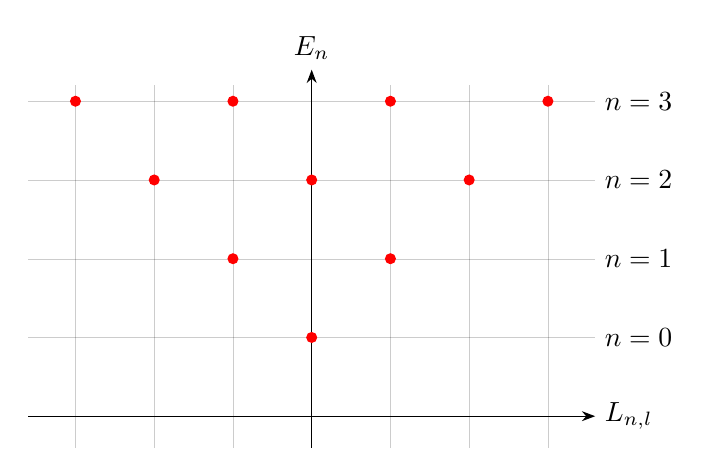
\begin{tikzpicture}
      \draw[-Stealth] (-3.6,0)--(3.6,0)node[right]{$L_{n,l}$};
      \draw[-Stealth] (0,-0.4)--(0,4.4)node[above]{$E_n$};      
      \begin{scope} \clip (-3.6,-0.4) rectangle (3.6,4.2);
        \draw[ultra thin, opacity=0.2] (1,-0.4)--(1,4.2);
        \draw[ultra thin, opacity=0.2] (2,-0.4)--(2,4.2);
        \draw[ultra thin, opacity=0.2] (3,-0.4)--(3,4.2);
        \draw[ultra thin, opacity=0.2] (-1,-0.4)--(-1,4.2);
        \draw[ultra thin, opacity=0.2] (-2,-0.4)--(-2,4.2);
        \draw[ultra thin, opacity=0.2] (-3,-0.4)--(-3,4.2);
        \draw[ultra thin, opacity=0.2] (-3.6,1)--(3.6,1);
        \draw[ultra thin, opacity=0.2] (-3.6,2)--(3.6,2);
        \draw[ultra thin, opacity=0.2] (-3.6,3)--(3.6,3);
        \draw[ultra thin, opacity=0.2] (-3.6,4)--(3.6,4);
      \end{scope}
      \draw(3.6,1)node[right]{$n=0$};
      \draw(3.6,2)node[right]{$n=1$};
      \draw(3.6,3)node[right]{$n=2$};
      \draw(3.6,4)node[right]{$n=3$};
      \fill[red](0,1)circle(2pt);
      \fill[red](1,2)circle(2pt);
      \fill[red](-1,2)circle(2pt);
      \fill[red](0,3)circle(2pt);
      \fill[red](2,3)circle(2pt);
      \fill[red](-2,3)circle(2pt);
      \fill[red](-3,4)circle(2pt);
      \fill[red](-1,4)circle(2pt);
      \fill[red](1,4)circle(2pt);
      \fill[red](3,4)circle(2pt);
    \end{tikzpicture}
    \caption{設問8の答え}
  \end{figure}


\end{enumerate}


\clearpage

\prb{2}{統計力学}

\begin{enumerate}

  \item 

  波動関数の位相部分は$e^{ikz}$なので,$\psi(z)=\psi(z+L)$であるためには
  \begin{equation}
    k_z
    =
    \frac{2\pi}{L}n_z
  \end{equation}
  でなければなりません.また,ハミルトニアンは
  \begin{equation}
    H(k_z)
    =
    \hbar vk_z
    \begin{pmatrix}
      1 & 0 \\
      0 & -1
    \end{pmatrix}
  \end{equation}
  なので、固有値は
  \begin{equation}
    \varepsilon_{k,1}
    =
    -
    \frac{2\pi \hbar v}{L}n_z
    ,\ 
    \varepsilon_{k,2}
    =
    +
    \frac{2\pi \hbar v}{L}n_z
  \end{equation}
  となります.図は省略.


  \item 

  エネルギーが$2\pi\hbar v/L$あたりに1つの状態が存在するので,
  \begin{equation}
    \Omega_0(\varepsilon)
    =
    \left\{
      \begin{alignedat}{1}
        \frac{L}{2\pi\hbar v}\varepsilon
        \quad
        &
        \quad
        (\varepsilon<\hbar vk_0)
        \\
        \frac{k_0 L}{2\pi}
        \quad
        &
        \quad
        (\varepsilon>\hbar vk_0)
      \end{alignedat}
    \right.
  \end{equation}
  となります.


  \item

  $\bm{k}\cdot\bm{\sigma}$の固有値は$\pm|\bm{k}|$なので,
  \begin{equation}
    \varepsilon_{k,1}
    =
    -\hbar v|\bm{k}|
    ,\ 
    \varepsilon_{k,2}
    =
    +\hbar v|\bm{k}|
  \end{equation}
  です.


  \item 

  波数は$z$成分同様
  \begin{equation}
    k_x
    =
    \frac{2\pi}{L}n_x
    ,\ 
    k_y
    =
    \frac{2\pi}{L}n_y
  \end{equation}
  と量子化されるので,エネルギーは
  \begin{equation}
    E_{n_x,n_y,n_z}
    =
    \frac{2\pi\hbar v}{L}
    \sqrt{n_x^2+n_y^2+n_z^2}
  \end{equation}
  です.したがって,$\Omega(\varepsilon)$は
  \begin{equation}    
    \frac{2\pi\hbar v}{L}
    \sqrt{n_x^2+n_y^2+n_z^2}
    \leq 
    \varepsilon
  \end{equation}
  つまり,
  \begin{equation}
    \sqrt{n_x^2+n_y^2+n_z^2}
    \leq
    \frac{\varepsilon L}{2\pi\hbar v}
  \end{equation}
  を満たす$(n_x,n_y,n_z)$の組だったので,それは半径が$\varepsilon L/2\pi\hbar v$の球で近似できて
  \begin{equation}
    \Omega(\varepsilon)
    =
    \frac{V}{6\pi^2\hbar^3 v^3}\varepsilon^3
  \end{equation}
  です.また,状態密度は
  \begin{equation}
    D(\varepsilon)
    =
    \dv{\Omega(\varepsilon)}{\varepsilon}
    =
    \frac{V}{2\pi^2\hbar^3 v^3}\varepsilon^2
  \end{equation}
  となります.


  \item 

  フェルミ統計なので
  \begin{equation}
    \sum_{n_{k,a}=0}^{1}
    e^{-\beta\varepsilon_{k,a}n_{k,a}}
    =
    1+e^{-\beta\varepsilon_{k,a}}
  \end{equation}
  であることに注意すると
  \begin{equation}
    \log \Xi(T,V)
    =
    \sum_{\bm{k}}\sum_{a=1}^{2}
    \log (1+e^{-\beta\varepsilon_{k,a}})
  \end{equation}
  となります.さて,総和を積分に書き直しますが,このとき,$\bm{k}$で総和をとるということは,$n_x,n_y,n_z$について和をとるということなので
  \begin{align}
    \log \Xi(T,V)
    &=
    \sum_{a=1}^{2}
    \sum_{n_x,n_y,n_z}
    \log (1+e^{-\beta\varepsilon_{k,a}})
    \nonumber
    \\
    &=
    \sum_{n_x,n_y,n_z}
    \log (1+e^{-\beta\varepsilon_{k,1}})
    +
    \sum_{n_x,n_y,n_z}
    \log (1+e^{-\beta\varepsilon_{k,2}})
    \nonumber
    \\
    &\sim
    \int_0^{\varepsilon_0}
    D(\varepsilon)
    \log (1+e^{\beta\varepsilon})
    \dd \varepsilon
    +
    \int_0^{\varepsilon_0}
    D(\varepsilon)
    \log (1+e^{-\beta\varepsilon})
    \dd \varepsilon
    \label{ans2_5}
  \end{align}
  です\footnote{
    $\varepsilon_{k,1}<0$なので,肩の符号に気をつけてください.
  }.したがって,$F(\varepsilon)=D(\varepsilon)\log (1+e^{\beta\varepsilon})(1+e^{-\beta\varepsilon})$となります.


  \item

  \eqref{ans2_5}の第2項については,部分積分を用いれば,公式を用いて計算しきることができます.積分区間を変更するために
  \begin{equation}    
    \int_0^{\varepsilon_0}
    D(\varepsilon)
    \log (1+e^{-\beta\varepsilon})
    \dd \varepsilon
    =
    \int_0^{\infty}
    D(\varepsilon)
    \log (1+e^{-\beta\varepsilon})
    \dd \varepsilon
    -
    \underbrace{
      \int_{\varepsilon_0}^{\infty}
      D(\varepsilon)
      \log (1+e^{-\beta\varepsilon})
      \dd \varepsilon
    }_{=G(\varepsilon_0)}
  \end{equation}
  とすれば,
  \begin{align}
    \int_0^{\infty}
    D(\varepsilon)
    \log (1+e^{-\beta\varepsilon})
    \dd \varepsilon
    &=
    \underbrace{
      \left[  
        \frac{V}{6\pi^2\hbar^3 v^3}\varepsilon^3
        \log (1+e^{-\beta\varepsilon})
      \right]_{0}^{\infty}
    }_{=0}
    +
    \frac{\beta V}{6\pi^2\hbar^3 v^3}
    \int_{0}^{\infty}
    \frac{\varepsilon^3}{e^{\beta\varepsilon}+1}
    \dd \varepsilon
    \nonumber
    \\
    &=
    \frac{\beta V}{6\pi^2\hbar^3 v^3}
    \cdot
    \frac{1}{\beta^4}\cdot\frac{7\pi^4}{120}
  \end{align}
  となります.一方の第1項ですが,部分積分すれば
  \begin{align}
    \int_{0}^{\varepsilon_0}
    D(\varepsilon)\log (1+e^{\beta\varepsilon})
    \dd \varepsilon
    =
    \left[  
      \frac{V}{6\pi^2\hbar^3 v^3}\varepsilon^3
      \log (1+e^{\beta\varepsilon})
    \right]_{0}^{\varepsilon_0}
    +
    \frac{\beta V}{6\pi^2\hbar^3 v^3}
    \int_{0}^{\varepsilon_0}
    \frac{\varepsilon^3}{e^{-\beta\varepsilon}+1}
    \dd \varepsilon
  \end{align}
  ですが,$\log(1+e^{\beta\varepsilon_0})\sim\beta\varepsilon_0$と近似すれば,発散項は
  \begin{equation}
    \left[  
      \frac{V}{6\pi^2\hbar^3 v^3}\varepsilon^3
      \log (1+e^{\beta\varepsilon})
    \right]_{0}^{\varepsilon_0}
    \sim
    \frac{\beta V}{6\pi^2\hbar^3 v^3}\varepsilon_0^4
  \end{equation}
  です.積分は
  \begin{equation}
    \int_0^{\varepsilon_0}
    \frac{\varepsilon^3}{e^{-\beta\varepsilon}+1}
    \dd \varepsilon
    =
    \int_0^{\varepsilon_0}
    \varepsilon^3
    \left(  
      1-e^{-\beta\varepsilon}+e^{-2\beta\varepsilon}-\cdots
    \right)
    \dd \varepsilon
    =
    \sum_{n=0}^{\infty}
    (-1)^n
    \int_0^{\varepsilon_0}
    \varepsilon^3 e^{-n\beta\varepsilon}
    \dd \varepsilon
  \end{equation}
  と書けるので
  \begin{equation}    
    \int_0^{\varepsilon_0}
    \varepsilon^3 e^{-n\beta\varepsilon}
    \dd \varepsilon
    =
    -\frac{6 e^{-n\beta\varepsilon_0}}{\beta^4 n^4}+\frac{6}{\beta^4
    n^4}-\frac{6 \varepsilon_0 e^{-n\beta\varepsilon_0}}{\beta^3
    n^3}-\frac{3 \varepsilon_0^2 e^{-n\beta\varepsilon_0}}{\beta^2
    n^2}-\frac{\varepsilon_0^3 e^{-n\beta\varepsilon_0}}{\beta  n}
  \end{equation}
  となり,
  \begin{equation}    
    \int_0^{\varepsilon_0}
    \frac{\varepsilon^3}{e^{-\beta\varepsilon}+1}
    \dd \varepsilon
    =
    \frac{\varepsilon_0^4}{4}
    +
    \sum_{n=1}^{\infty}
    (-1)^n
    \left[ 
      -\frac{6 e^{-n\beta\varepsilon_0}}{\beta^4 n^4}+\frac{6}{\beta^4
      n^4}-\frac{6 \varepsilon_0 e^{-n\beta\varepsilon_0}}{\beta^3
      n^3}-\frac{3 \varepsilon_0^2 e^{-n\beta\varepsilon_0}}{\beta^2
      n^2}-\frac{\varepsilon_0^3 e^{-n\beta\varepsilon_0}}{\beta  n}
    \right]
  \end{equation}
  です.したがって,$n=1$のときは,$e^{-\beta\varepsilon_0}\sim 0$より$6/\beta^4$のみを拾ってきて,残りの$n>2$の項は無視して
  \begin{equation}
    \int_0^{\varepsilon_0}
    \frac{\varepsilon^3}{e^{-\beta\varepsilon}+1}
    \dd \varepsilon
    \sim
    \frac{\varepsilon_0^4}{4}
    -
    \frac{6}{\beta^4}    
  \end{equation}
  とします\footnote{
    もっとスマートな近似があるといいのですが,今回はゴリゴリ計算して評価しました.(Mathematicaを持ち込みたいです.)
  }.以上より,
  \begin{equation}
    \log \Xi[T,V]
    =
    \frac{V}{6\pi^2\hbar^3 v^3}
    \cdot
    \frac{1}{\beta^3}\cdot\frac{7\pi^4}{120}
    +
    \frac{\beta V}{6\pi^2\hbar^3 v^3}\varepsilon_0^4
    +
    \frac{\beta V}{6\pi^2\hbar^3 v^3}
    \left[  
      \frac{\varepsilon_0^4}{4}
      -
      \frac{6}{\beta^4}    
    \right]
    +
    G(\varepsilon_0)
  \end{equation}
  です.


  \item 

  エネルギーは
  \begin{align}
    E
    &=
    -\pdv{}{\beta}
    \log\Xi[T,V]
    \nonumber
    \\
    &=
    -
    \frac{5V\varepsilon_0^4}{24\pi^2\hbar^3v^3}
    -
    \frac{(720-7\pi^4)k_B^4V}{240\pi^2\hbar^3v^3}T^4
  \end{align}
  であり,
  \begin{equation}
    C_V
    =
    -
    \frac{(720-7\pi^4)k_B^4V}{60\pi^2\hbar^3v^3}T^3    
    \propto
    T^3
  \end{equation}
  となります.


  \item 

  一般に理想フェルミ理想気体の物理量を低温展開で求めると,$T$について奇数次の項は積分でキャンセルされます.つまり,エネルギーは定数を除けば$T$の最低次数は$2$.したがって,比熱は$T$の1次.今回の場合は,そもそもスピンという内部自由度があったため,状態密度が変化し,結果が異なっているのだと思います.


\end{enumerate}



\clearpage

\prb{3}{電磁気学}

\begin{enumerate}

  \item 

  ちゃんと成分で書いてみると
  \begin{align}
    |\bm{r}-\bm{r}_0|
    &=
    \sqrt{(x-x_0)^2+(y-y_0)^2+(z-z_0)^2}
    \nonumber
    \\
    &\sim
    \sqrt{r^2-2\bm{r}\cdot\bm{r_0}}
    \nonumber
    \\
    &=
    r\sqrt{1-2\hat{\bm{r}}\cdot\frac{\bm{r}_0}{r}}
    \nonumber
    \\
    &\sim
    r
    \left( 1-\hat{\bm{r}}\cdot\frac{\bm{r}_0}{r} \right)
  \end{align}
  となります.ただし,$\hat{\bm{r}}$は単位ベクトル.


  \item 

  ポテンシャルは
  \begin{equation}
    \phi(\bm{r})
    =
    \frac{e}{4\pi\varepsilon_0}
    \cdot
    \frac{1}{\sqrt{x^2+(y-d/2)^2+z^2}}
    -
    \frac{e}{4\pi\varepsilon_0}
    \cdot
    \frac{1}{\sqrt{x^2+(y+d/2)^2+z^2}}
  \end{equation}
  ですが,
  \begin{equation}
    \frac{1}{\sqrt{x^2+(y\pm d/2)^2+z^2}}
    \sim
    \frac{1}{r}\left( 1\pm \frac{yd}{r^2} \right)^{-1/2}
    \sim
    \frac{1}{r}
    \left( 1\mp\frac{yd}{2r^2} \right)
  \end{equation}
  となっているので,
  \begin{equation}
    \phi(\bm{r})
    \sim
    \frac{e}{4\pi\varepsilon_0}
    \cdot
    \frac{yd}{r^3}
  \end{equation}
  です.

  
  \item 

  $1/r^3$を$x$で微分してみると
  \begin{equation}
    \pdv{}{x}\left(\frac{1}{r^3}\right)
    =
    -\frac{3x}{r^5}
  \end{equation}
  となるので
  \begin{equation}
    E_x
    =
    \frac{e}{4\pi\varepsilon_0}
    \cdot
    \frac{3xyd}{r^5}
    ,\ 
    E_z
    =
    \frac{e}{4\pi\varepsilon_0}
    \cdot
    \frac{3yzd}{r^5}
  \end{equation}
  です.一方で,$y$については
  \begin{equation}
    E_y
    =
    \frac{e}{4\pi\varepsilon_0}
    \cdot
    \frac{3y^2d}{r^5}
    -
    \frac{e}{4\pi\varepsilon_0}
    \cdot
    \frac{d}{r^3}
  \end{equation}
  となります.


  \item

  $x,z=0$なので,$\bm{E}$は$E_y$しか残っていません.$r=y$に気をつければ,
  \begin{equation}
    U
    =
    -
    p\sin\theta
    \cdot
    \frac{e}{4\pi\varepsilon_0}
    \cdot
    \frac{2d}{y^3}
  \end{equation}
  です.


  \item 

  $\theta=\pi/2$.


  \item 

  電荷密度分布は
  \begin{equation}
    \rho(\bm{r})
    =
    \delta(x)\delta(z)
    \left(  
      2e\delta(y)
      -
      e(\delta(y-d/2)+\delta(y+d/2))
    \right)
  \end{equation}
  として計算します.ここで,$\delta(x)$や$\delta(z)$がくくりだされていることに注意しましょう.つまり,$\rho(\bm{r})$に$x$や$z$をかけて積分すると$0$になってしまうので,$p_2$や$Q_{22}$のみを計算すればよいことになります.まずは$p_2$から計算してみると
  \begin{align}
    p_2
    &=
    \int
    y'\rho(\bm{r}')\dd^3 \bm{r}'
    \nonumber
    \\
    &=
    \frac{ed}{2}-\frac{ed}{2}
    =
    0
  \end{align}
  となります.一方で,$Q_{22}$は
  \begin{align}
    Q_{22}
    &=
    \frac{1}{2}
    \int
    (2{y'}^2-({x'}^2+{z'}^2))
    \rho(\bm{r}')
    \dd^3 \bm{r}'
    \nonumber
    \\
    &=
    -\frac{ed^2}{2}
  \end{align}
  です.


  \item 

  ポテンシャルは
  \begin{align}
    \varphi(\bm{r})
    &=
    \frac{1}{4\pi\varepsilon_0}
    \cdot
    \frac{y^2 Q_{22}}{r^5}
    \nonumber
    \\
    &=
    -
    \frac{e}{4\pi\varepsilon_0}
    \cdot
    \frac{d^2 y^2}{r^5}
  \end{align}
  です.したがって,
  \begin{equation}
    E_x
    =
    -\frac{5ed^2}{4\pi\varepsilon_0}
    \frac{xy^2}{r^7}
    ,\ 
    E_z
    =
    -\frac{5ed^2}{4\pi\varepsilon_0}
    \frac{zy^2}{r^7}
  \end{equation}
  であり,
  \begin{equation}    
    E_y
    =
    -\frac{5ed^2}{4\pi\varepsilon_0}
    \frac{y^3}{r^7}
    +
    -\frac{ed^2}{2\pi\varepsilon_0}
    \frac{y}{r^5}
  \end{equation}
  です.


  \item 

  (c1)では,$Q_{22}=-ed^2/2$なので
  \begin{align}
    U_{\text{(c1)}}
    &=
    \frac{ed^2}{6}
    \left.\pdv{E_y}{y}\right|_{\bm{r}=(0,a,0)}
    \nonumber
    \\
    &=    
    \frac{ed^2}{6}
    \left.\left(  
      -\frac{35y^4}{r^9}
      +
      \frac{20y^2}{r^7}
      -
      \frac{1}{r^5}
    \right)\right|_{\bm{r}=(0,a,0)}    
    =
    \frac{ed^2}{6}
    \frac{ed^2}{4\pi\varepsilon_0}
    \frac{16}{a^5}
    \ 
    (>0)
  \end{align}
  です.一方で,(c2)では$Q_{11}=-ed^2/2$なので\footnote{
    軸を変更しただけなので,$Q_{11}$だけが値をもつことになります.
  },
  \begin{align}
    U_{\text{(c1)}}
    &=
    \frac{ed^2}{6}
    \left.\pdv{E_x}{x}\right|_{\bm{r}=(0,a,0)}
    \nonumber
    \\
    &=    
    -
    \frac{ed^2}{6}
    \frac{5ed^2}{4\pi\varepsilon_0}
    \frac{1}{a^5}
    \ 
    (<0)
  \end{align}
  です.したがって,(c2)の系のほうがエネルギーが小さいです.


\end{enumerate}


\clearpage

\prb{4}{数学}

\begin{enumerate}

  \item 

  \begin{enumerate}
    \item 

    $x=\cos\theta,\ y=\sin\theta$.

    
    \item 

    $z^{n}=\cos n\theta+i\sin n\theta$なので,
    \begin{equation}
      \cos n\theta
      =
      \frac{z^n + 1/z^{n}}{2}
      ,\ 
      \cos\theta
      =
      \frac{z+1/z}{2}
    \end{equation}
    と変換されるので
    \begin{equation}
      I
      =
      \frac{1}{ib}
      \int_{C}
      \frac{z^{2n}+1}{z^2+2(a/b)z+1}\frac{1}{z^n}\dd z
    \end{equation}
    となります.経路は半径1の円周です.


    \item 

    $b<a$であることに気をつければ,$|z|<1$であるのは
    \begin{equation}
      z
      =
      0
      ,
      \lambda_{+}
    \end{equation}
    です\footnote{
      次の点
      $$
        \lambda_{-}
        =
        -\frac{a}{b}
        -
        \frac{a}{b}
        \sqrt{
          1-\left( \frac{b}{a} \right)^2
        }
      $$
      も極の候補ですが,$|\lambda_{-}|>1$なので,今回の積分の極ではあり得ません.また,$\lambda_{+}$の絶対値ですが,$\lambda_{\pm}<0$なので
      $$
        -\frac{a}{b}
        +
        \frac{a}{b}
        \sqrt{
          1-\left( \frac{b}{a} \right)^2
        }
        >
        -1        
      $$
      を示せば良いことが分かります.ここまで分かれば,この不等式が成立していることをチェックするだけです.(ちょっと移項して,2乗すればOK.)
    }.ただし,
    \begin{equation}
      \lambda_{\pm}
      \equiv
      -\frac{a}{b}
      \pm
      \frac{a}{b}
      \sqrt{
        1-\left( \frac{b}{a} \right)^2
      }      
    \end{equation}
    としました.


    \item 

    $n=2$のときは
    \begin{equation}
      I
      =
      \frac{1}{ib}
      \int
      \frac{z^4+1}{z^2(z^2+2(a/b)z+1)}\dd z
    \end{equation}
    です.被積分関数を
    \begin{equation}
      f(z)
      \equiv
      \frac{z^4+1}{z^2(z^2+2(a/b)z+1)}
    \end{equation}
    とおいて,留数を求めます.$z=0$は2位の極なので
    \begin{align}
      \Residue[f,0]
      &=
      \lim_{z\rightarrow 0}
      \dv{}{z}
      \left(  
        \frac{z^4+1}{z^2+2(a/b)z+1}
      \right)
      \nonumber
      \\
      &=
      \lim_{z\rightarrow 0}
      \frac{
        4z^3(z^2+2(a/b)z+1)
        -
        (z^4+1)(2z+2(a/b))
        }{(z^2+2(a/b)z+1)^2}
        =
        -\frac{2a}{b}
    \end{align}
    となります.$z=\lambda_{+}$のほうは,1位の極なので
    \begin{equation}
      \Res[f,\lambda_{+}]
      =
      \frac{\lambda_{+}^4+1}{\lambda_{+}^2(\lambda_{+}-\lambda_{-})}
    \end{equation}
    となり,積分は
    \begin{equation}
      I
      =
      \frac{2\pi}{b}
      \left[  
        -
        \frac{2a}{b}
        +
        \frac{\left( -\dfrac{a}{b}+\dfrac{a}{b}\sqrt{1-\left( \dfrac{b}{a} \right)^2} \right)^4+1}{\left( -\dfrac{a}{b}+\dfrac{a}{b}\sqrt{1-\left( \dfrac{b}{a} \right)^2} \right)^2\cdot\dfrac{2a}{b}\sqrt{1-\left( \dfrac{b}{a} \right)^2}}
      \right]
    \end{equation}
    となります
    \footnote{
      整理しようとMathematicaにもかけてみましたが,うまくいきませんでした.一応,Mathematicaにダイレクトに解かせた結果は
      $$
        I
        =
        \frac{2b^2\pi}{2a^3-2ab^2+2a^2\sqrt{a^2-b^2}-b^2\sqrt{a^2-b^2}}
      $$
      で,具体的に$a,b$の値をいくつか代入した結果はあっていたので,たぶんこれで良いと思います.
    }.


  \end{enumerate}


  \item 

  \begin{enumerate}

    \item 

    $(VXV^{-1})^{n}=VX^{n}V^{-1}$なので.

    
    \item 

    固有方程式は
    \begin{equation}
      \begin{vmatrix}
        \lambda-\frac{1}{\sqrt{2}} & 0 & 0 & \frac{1}{\sqrt{2}} \\
        0 & \lambda-1 & 0 & 0 \\
        0 & 0 & \lambda+1 & 0 \\
        -\frac{1}{\sqrt{2}} & 0 & 0 & \lambda-\frac{1}{\sqrt{2}}
      \end{vmatrix}
      =
      0
    \end{equation}
    なので,余因子展開をすれば
    \begin{equation}
      (\lambda+1)(\lambda-1)(\lambda^2-\sqrt{2}\lambda+1)
      =
      0
    \end{equation}
    となり,固有値は
    \begin{equation}
      \lambda
      =
      \pm 1
      ,\ 
      \frac{1\pm i}{\sqrt{2}}
    \end{equation}
    となります.固有ベクトルを求めると
    \begin{equation}
      u_1
      =
      \begin{pmatrix}
        0 \\
        1 \\
        0 \\
        0
      \end{pmatrix}
      ,\ 
      u_2
      =
      \begin{pmatrix}
        0 \\
        0 \\
        1 \\
        0
      \end{pmatrix}
      ,\ 
      u_3
      =
      \frac{1}{\sqrt{2}}
      \begin{pmatrix}
        1 \\
        0 \\
        0 \\
        -i
      \end{pmatrix}
      ,\ 
      u_4
      =
      \frac{1}{\sqrt{2}}
      \begin{pmatrix}
        1 \\
        0 \\
        0 \\
        i
      \end{pmatrix}
    \end{equation}
    となります.


    \item 

    \begin{equation}
      U
      =
      \begin{pmatrix}
        0 & 0 & 1/\sqrt{2} & 1/\sqrt{2} \\
        1 & 0 & 0 & 0 \\
        0 & 1 & 0 & 0 \\
        0 & 0 & -i/\sqrt{2} & i/\sqrt{2}
      \end{pmatrix}
      ,\ 
      D
      =
      \begin{pmatrix}
        1 & & & \\
          & -1 & & \\
          & & \frac{1+i}{\sqrt{2}} & \\
          & & & \frac{1-i}{\sqrt{2}}
      \end{pmatrix}
      .
    \end{equation}


    \item 

    $A^n$を計算すると,
    \begin{align}
      A^n
      &=
      \begin{pmatrix}
        0 & 0 & 1/\sqrt{2} & 1/\sqrt{2} \\
        1 & 0 & 0 & 0 \\
        0 & 1 & 0 & 0 \\
        0 & 0 & -i/\sqrt{2} & i/\sqrt{2}
      \end{pmatrix}    
      \begin{pmatrix}
        1 & & & \\
          & (-1)^n & & \\
          & & e^{in\pi/4} & \\
          & & & e^{-in\pi/4}
      \end{pmatrix} 
      \begin{pmatrix}
        0 & 1 & 0 & 0 \\
        0 & 0 & 1 & 0 \\
        1/\sqrt{2} & 0 & 0 & i/\sqrt{2} \\
        1/\sqrt{2} & 0 & 0 & -i/\sqrt{2}
      \end{pmatrix}   
      \nonumber
      \\
      &=
      \begin{pmatrix}
        \cos\dfrac{n\pi}{4} & 0 & -\sin \dfrac{n\pi}{4} \\
        0 & 1 & 0 & 0 \\
        0 & 0 & (-1)^n & 0 \\
        \sin\dfrac{n\pi}{4} & 0 & 0 & -\cos\dfrac{n\pi}{4}
      \end{pmatrix}  
    \end{align}
    となるので,
    \begin{equation}
      e^{itA}
      =
      \sum_{n=0}^{\infty}
      \frac{(it)^n}{n!}
      \begin{pmatrix}
        \cos\dfrac{n\pi}{4} & 0 & -\sin \dfrac{n\pi}{4} \\
        0 & 1 & 0 & 0 \\
        0 & 0 & (-1)^n & 0 \\
        \sin\dfrac{n\pi}{4} & 0 & 0 & -\cos\dfrac{n\pi}{4}
      \end{pmatrix}  n   
    \end{equation}
    です.


  \end{enumerate}


\end{enumerate}


\end{document}
